\chapter{Diseño e implementación} % Main chapter title

\label{Chapter3} % Change X to a consecutive number; for referencing this chapter elsewhere, use \ref{ChapterX}


\section{Descripción del sistema}


\textbf{PARAFRASEAR EL PRIMER PARRAFO PORQUE SE REPITE CON LA MOTIVACION DEL PROYECTO !}

El \textit{SAL/T}, según sus siglas, Sistema de Aislamiento Limitado o Total, es un sistema que le permitirá al conductor la activación y desactivación del modo aislado limitado. En este modo, el equipo permite la circulación de la formación al desactivar las señales de corte de tracción y freno de emergencia generadas por los otros subsistemas. Para que esta operación se realice de forma segura, se debe monitorear la velocidad de la formación tal que sea posible evitar que supere cierto valor máximo. 
Se considera un sistema crítico debido a que, en caso de fallar, puede ocasionar lesiones o muertes de personas, dañar el medio ambiente y/o generar grandes pérdidas materiales.

En trabajos anteriores se desarrollaron las primeras cinco fases de catorce que componen el ciclo de vida según la norma \textit{UNE-EN 50126}, centradas en el relevamiento de la necesidad y la obtención de los requerimientos técnicos del sistema.

En la actualidad, existe un prototipo de este sistema que fue finalizado en el año 2019, del cual, en lo que respecta al \textit{firmware}, se propone realizar la migración a un microcontrolador de la familia \textit{Cortex} tipo M con mayor soporte al actual y que cuente con funcionalidades de seguridad.  

Por otro lado, tal como se puede observar en el margen inferior derecho de la figura 1, se plantea el desarrollo de una central operativa. Se trata de una plataforma web que cuenta con una unidad lógica de compartición y empaquetado de software posibilitando la administación, la configuración y el monitoreo en tiempo real de la información recibida y transmitida por parte de cada dispositivo SAL/T. 


\newpage
En caso de ser necesario, a partir de la activación de una señal crítica provista por el artefacto \textit{Hasler} \footnote{ es un sistema electromecánico que registra los eventos de velocidad del material rodante, la señal de anuncio y la señal de frenado automático.
}  que se encuentra instalado en cada formación ferroviaria, un operario puede accionar alguno de los comandos que se listan a continuación:


\begin{itemize}
	\item \textbf{Modo aislado total}: se habilita la tracción y se libera el freno de emergencia, independientemente de cualquier condición. 

    \item \textbf{Modo coche en deriva}: se corta la tracción y se libera el freno de emergencia, independientemente de cualquier condición. 

    \item \textbf{Modo parada total}: se corta la tracción y se aplica el freno de emergencia, independientemente de cualquier condición. 
    
    \item \textbf{Modo intermitente}: se habilita la tracción y se aplica el freno de emergencia en ciclos de tiempo configurables. 

    \item Anulación de comandos remotos vigentes.

\end{itemize}


Para el seguimiento de las variables, publicadas por cada dispositivo SAL/T, que permiten la visualización en la plataforma, se realiza la suscripción a un tópico del \textit{broker} \textit{MQTT} y se registra la información indexada en la base de datos de un servidor. En consecuencia, resulta de extrema importancia que la comunicación a través de \textit{MQTT} opere sobre el protocolo de encriptación \textit{SSL/TSL}, de modo que se exponga un considerable nivel de seguridad; de igual manera, es necesaria la utilización de certificados para el acceso a la lectura y la escritura en la base de datos.  

Así mismo, es necesario que la página web ofrezca la configuración de los parámetros de cada dispositivo conectado a la formación ferroviaria, la administración de los roles y la autenticación de los usuarios.

\begin{figure}[htpb]
\centering 
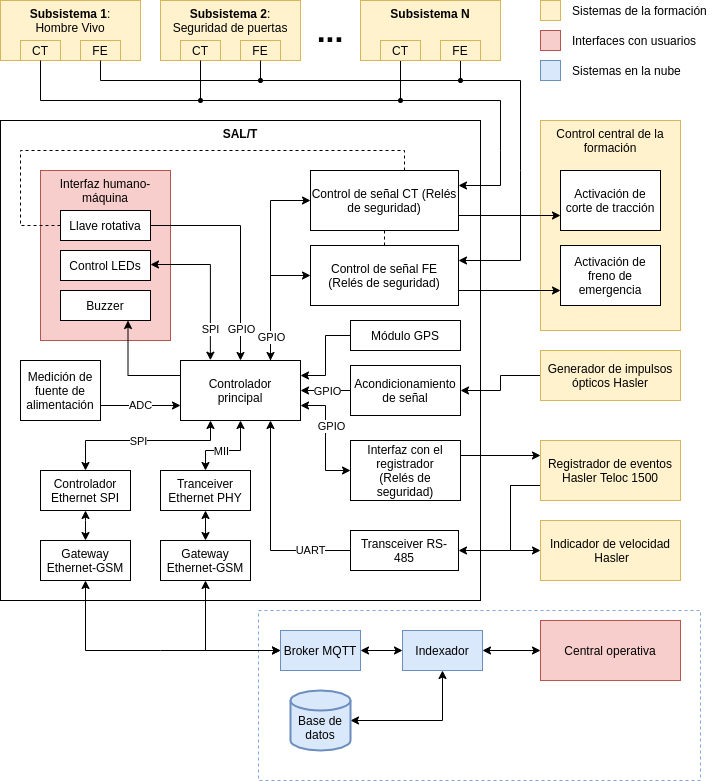
\includegraphics[width=.8\textwidth]{Figures/diagrama_salt_con_central.png}
\caption{Diagrama en bloques del sistema SALT.}
\label{fig:diagBloques}
\end{figure}

\subsection{Comunicación device & backend}

MQTT

Ver cuanto se repite con el ultimo parrafo de arriba.

\subsection{Comunicación backend & frontend}

HTTP

Ver cuanto se repite con el ultimo parrafo de arriba.


\section{Arquitectura del sistema}


\textbf{PARAFRASEAR EL PRIMER PARRAFO PORQUE SE REPITE CON LA MOTIVACION DEL PROYECTO !}

A partir de los modelos más relevantes que se encuentran establecidos para el desarrollo e implementación de aplicaciones de software se consideran el \textit{stack web} y el \textit{stack IoT}. A pesar de las similitudes entre ambos, en la aplicación el \textit{stack web} emplea el protocolo \textit{HTTP} \cite{b5} mientras que el \textit{stack IoT} utiliza el protocolo \textit{MQTT} \cite{b6}; siendo este último el más adecuado para escenarios donde son limitados los recursos como el ancho de banda y el consumo de energía.

En especial, el protocolo \textit{MQTT} dispone de mensajes más livianos y además es posible transmitir y/o recibir datos en formato binario sin la necesidad de una codificación previa. También, este protocolo permite asignar niveles de calidad de servicio (\textit{QoS}) \cite{b7} a los mensajes transmitidos, resultando una característica primordial en aplicaciones donde la probabilidad de pérdidas de paquetes es considerable.

La \textbf{figura X} presenta la estratificación de las capas, según el \textit{stack IoT}, que son detalladas a lo largo de esta sección.


\textbf{AGREGAR NUEVA FIGURA SUPER GENERAL DEL STACK IOT CON SUS CAPAS}


\subsection{Capa de dispositivos}

Sobre la base de un prototipo del Sistema de Aislamiento Limitado o Total, \textit{SAL/T} \cite{b1}, se desarrolló mediante el kit de desarrollo \textit{Nucleo F429} \cite{b8}, un cliente \textit{MQTT} que permite la publicación de la velocidad de la formación y de los parámetros provistos por los subsistemas de falla, entre otras variables; y llegado el caso, el dispositivo pueda realizar la lectura de diferentes parámetros configurables.

\subsection{Capa de conectividad}

Para la comunicación entre los dispositivos \textit{SAL/T} y la capa de almacenamiento se emplea un \textit{Broker MQTT} que oficia de orquestador entre el cliente, el dispositivo \textit{SAL/T} que publica los mensajes y \textit{Apache Kafka} \cite{b9}, un sistema distribuido que efectúa la lectura de la información y su posterior procesamiento. 

Dado que los mensajes intercambiados entre las partes contienen información sensible, se ha optado por agregar la capa de seguridad \textit{TLS} \cite{b10}. En este sentido, resulta indispensable utilizar el certificado \textit{X509} \cite{b11} para prevenir ataques del tipo \textit{adversary-in-the-middle} \cite{b12} y los certificados emitidos por autoridades reconocidas.


\subsection{Capa de almacenamiento}

La capa de almacenamiento se encuentra constituida por el sistema distribuido \textit{Kafka} que se encarga de almacenar los datos de la aplicación. Entre ellos se destacan los mensajes MQTT enviados por los dispositivos SAL/T, como también la información referida a las formaciones y a los SAL/T que las ocupan. Además, se tienen servicios de procesamiento de datos que se encargan de adaptar la información de los tópicos en datos que posteriormente serán consumidos por los servicios que integran la capa superior.

Por otro lado, se tiene una base de datos relacional \textit{PostgreSQL} \cite{b13} para el almacenamiento de los datos provenientes del servicio de autenticación y el motor que facilita la interacción con la plataforma web. Los conectores se encargan de insertar los datos que se quieran disponer a la capa de visualización.


En la figura \textbf{devicesTrainEntity} se observa el modelo de datos que representa a los dispositivos SAL/T, las formaciones y las entidades. 
El primero cuenta con un identificador del dispositivo en el sistema, el estado de operación y una referencia al tren en el que se desplegó el artefacto. 
El modelo de la formación está enriquecido con la entidad a la que pertenece y el número de serie del tren. 
Por último, las entidades están compuestas por nombre y descripción.
En la figura \textbf{devicesSubsystems} se aprecian los subsistemas de fallas relacionados con el dispositivo SAL/T. Su modelo está integrado con el nombre del subsistema, el identificador del dispositivo al que está asociado y el estado actual del mismo. 

\subsection{Capa de interacción}

La capa de interacción se encuentra conformada por tres unidades. Por un lado, se ha desarrollado en el lenguaje \textit{Kotlin} \cite{b14} en conjunto con el \textit{framework} \textit{Ktor} \cite{b15}, un microservicio de autenticación donde es posible la gestión de los usuarios con sus respectivos roles y también el \textit{backend}. Entre sus tareas principales se encuentran las relacionadas con el protocolo \textit{MQTT} para la actualización de los certificados que brindan seguridad a las comunicaciones, mediante el uso de la capa de seguridad \textit{TLS}, y la indexación de los eventos que se publiquen en tiempo real; como la configuración general que permite el funcionamiento integral de los servicios y módulos dispuestos en el sistema. \\

Además, se dispone del motor \textit{Hasura} \cite{b16}, el cual se encuentra conectado a una base de datos relacional (\textit{PostgreSQL}) basado en el lenguaje de consulta estructurado \textit{SQL} \cite{b17}, que permite exponer una \textit{API GraphQL} \cite{b18} a aquellos clientes que deseen obtener una visualización del modelo de datos propuesto en que se conjuga la información de cada formación ferroviaria con su correspondiente dispositivo \textit{SAL/T} y diseño destinado al \textit{frontend}. Más aún, el enlace permite realizar modificaciones y hasta remociones de las columnas propuestas en las tablas de cada esquema dentro de la base de datos.


\subsection{Capa de visualización}

En esta capa se ha utilizado el lenguaje de programación \textit{TypeScript} \cite{b19} junto con la biblioteca gráfica \textit{React} \cite{b20} para brindar una web reactiva en la que se elaboraron los formularios, las tablas y los paneles a partir de la explotación de la información almacenada en la base de datos. Cabe destacar que la plataforma web se encuentra condicionada por el rol y la entidad a la que pertenece cada usuario, de modo que, cada formación ferroviaria tendrá un operador asignado, el cual podrá modificar los parámetros correspondientes con el dispositivo asociado.

En la figura \textbf{dashboard} se puede apreciar el panel de control de la central operativa al que tendrán acceso los operadores de cada entidad.
En el mismo se observan distintas tarjetas con el estado de cada subsistema de fallas y del tren, como así también un velocímetro que informa la velocidad de la formación.


\section{Arquitectura de datos}

Para crear la estructura de la base de datos SQL, se realiza un análisis detallado del sistema y se identifican las principales entidades: la formación ferroviaria, los subsistemas de falla y las áreas. Toda la información de estas entidades se nuclea en la entidad tren, la cual representa una formación ferroviaria con todos sus subsistemas y áreas asociadas. A partir del modelado de estas entidades y sus atributos correspondientes, se definen las relaciones entre ellas y se establecen las claves primarias y foráneas.


Para visualizar de manera más clara la estructura de la base de datos y sus relaciones, se utiliza el diagrama UML (Lenguaje de Modelado Unificado). En la siguiente figura se muestra el diagrama UML de la base de datos, donde se pueden observar las diferentes entidades, sus atributos y relaciones. A partir de este diagrama se procede a crear las tablas en la base de datos SQL y a definir sus columnas y restricciones, garantizando así la integridad de los datos y el correcto funcionamiento del sistema.


\textbf{CONTINUAR CON EL DIAGRAMA UML CONECTANDO LAS ENTIDADES  \\ VER Figures/salt\_uml\_drawio}
\url{https://app.diagrams.net/}


\subsection{Entidades del modelo de datos}


\textbf{COMENTAR SI ES QUE LAS HAY, PARTICULARIDADES SOBRE CADA UNA DE LAS ETIDADES DEL SISTEMA Y CADA TABLA DEL DIAGRAMA UML}

 
\subsubsection{Schema auth\_service}

\begin{itemize}

\item \textbf{credentials}: Esta tabla almacena las credenciales de los usuarios para acceder al sistema. Tiene una clave foránea a la tabla \textbf{auth\_service users} y es referenciada por la tabla \textbf{auth\_service roles}.

\item \textbf{roles}: Esta tabla almacena los roles de los usuarios. Tiene una clave foránea a la tabla \textbf{auth\_service users} y es referenciada por la tabla \textbf{enums roles}.

\item \textbf{users}: Esta tabla almacena la información básica de los usuarios del sistema. Es referenciada por la tabla \textbf{auth\_service credentials} y la tabla \textbf{public users}.

\end{itemize}


\subsubsection{Schema enums}

\begin{itemize}

  \item \textbf{device status}: Esta tabla almacena los estados posibles para los dispositivos. Es referenciada por la tabla \textbf{public devices}.

  \item \textbf{events}: Esta tabla almacena los tipos de eventos posibles. Es referenciada por la tabla \textbf{public internal events}.

  \item \textbf{fail system}: Esta tabla almacena los sistemas de falla posibles. Es referenciada por la tabla \textbf{public remote events} y la tabla \textbf{public subsystems}.

  \item \textbf{roles}: Esta tabla almacena los roles posibles para los usuarios del sistema. Es referenciada por la tabla \textbf{auth\_service roles}.

\end{itemize}


\subsubsection{Schema public}

\begin{itemize}

\item \textbf{devices}: Esta tabla almacena información sobre los dispositivos del sistema. Tiene una clave foránea a la tabla \textbf{public train} y es referenciada por la tabla \textbf{public remote events} y la tabla \textbf{public internal events}.

\item \textbf{entities}: Esta tabla almacena información sobre las entidades del sistema. Es referenciada por la tabla \textbf{public train}.

\item \textbf{internal events}: Esta tabla almacena información sobre los eventos internos del sistema. Tiene claves foráneas a las tablas \textbf{public devices}, \textbf{enums events} y \textbf{public users}.

\item \textbf{remote events}: Esta tabla almacena información sobre los eventos remotos del sistema. Tiene una clave foránea a la tabla \textbf{public devices} y es referenciada por la tabla \textbf{enums fail system}.

\item \textbf{subsystems}: Esta tabla almacena información sobre los subsistemas del sistema. Tiene una clave foránea a la tabla \textbf{public devices} y es referenciada por la tabla \textbf{enums fail system}.

\item \textbf{train}: Esta tabla almacena información sobre los trenes del sistema. Tiene una clave foránea a la tabla \textbf{public entities} y es referenciada por la tabla \textbf{public devices}.

\item \textbf{user data}: Esta tabla almacena información adicional de los usuarios del sistema. Es referenciada por la tabla \textbf{public users}.

\item \textbf{users}: tabla que contiene información de los usuarios. Tiene una relación de clave externa con la tabla entities.


\end{itemize}






\section{Seguridad del sistema}

\subsection{Protocolo HTTPS}

security layer

jwt

\textbf{Referencia - pag 44}
https://lse-posgrados-files.fi.uba.ar/tesis/LSE-FIUBA-Trabajo-Final-CEIoT-Pedro-Rosito-2021.pdf


\subsection{MQTT v5.0}

payload encryption



\section{Desarrollo del frontend}

\textbf{AGREGAR UNA BREVE INTRO SOBRE QUE SE EXPONDRA AQUI}
\textit{tipos de clientes, apollo client, codegen, }

\subsection{Estructura del cliente web}

\begin{enumerate}

  \item index html

  \item main tsx 

  \item react router -> pages

\end{enumerate}


\subsection{Páginas}

\textbf{HABLAR DE CADA PAGINA A PARTIR DE UNA IMAGEN DONDE SE MUESTRE EL SIDEBAR}

\textit{dashboard, sign in, configuration, entities, trains, subsystems of each train, logs, etc}

\subsubsection{Login}

\textbf{hablar sobre jwt}
\textit{Referecia - bastian pag 48}

\textbf{add figure}


\subsubsection{Tabla de trenes+salt}

\textbf{add figure}


\subsubsection{Tabla de usuarios}

\textbf{add figure}


\subsubsection{dashboard}

\textbf{add figure}

\subsection{Modales}

\textit{crear: usuario, tren, dispositivo ; configuracion: sub sistemas de seguridad, etc}





\section{Desarrollo del backend}


A partir del uso de archivo docker-compose, que se ejecuta en un entorno Docker, para proporcionar el conjunto completo de servicios para enviar, recibir y almacenar los datos a través de diferentes protocolos. Cada servicio se ejecuta en su propio contenedor y se conecta a los otros servicios según el siguiente formato:


\textbf{AGREGAR IMAGEN DEL ENTORNO DOCKER CON SUS CONTENEDORES Y CONEXIONES }
\url{https://www.gotoiot.com/pages/articles/docker_intro/index.html}
\url{https://www.gotoiot.com/pages/articles/docker_intro/images/image2.png}


\begin{itemize}

  \item mosquitto: es un servidor MQTT de código abierto que se utiliza para enviar y recibir mensajes. Se utiliza la imagen "eclipse-mosquitto" y se mapea el puerto 1883 en el host al puerto 1883 en el contenedor. También se montan dos volúmenes, uno para la configuración del servidor y otro para los datos.

  \item hasura: es un motor de GraphQL que proporciona una API para interactuar con una base de datos. Se utiliza la imagen "hasura/graphql-engine:v2.1.0" y se mapea el puerto 8080 en el host al puerto 8080 en el contenedor. Se configuran varias variables de entorno, incluyendo la URL de la base de datos y el secreto de administrador. También depende del servicio "postgres".

  \item postgres: es una base de datos relacional que se utiliza para almacenar datos. Se utiliza la imagen "postgres:13" y se mapea el puerto 5432 en el host al puerto 5432 en el contenedor. Se configuran varias variables de entorno, incluyendo el nombre de la base de datos, el nombre de usuario y la contraseña. También se monta un volumen para almacenar los datos de la base de datos.

  \item zookeeper: es un servicio que se utiliza para coordinar los nodos de Kafka. Se utiliza la imagen "confluentinc/cp-zookeeper:6.2.4" y se configura el puerto de cliente en 2181.

  \item kafka: es un servicio de mensajería de código abierto que se utiliza para enviar y recibir mensajes. Se utiliza la imagen "confluentinc/cp-kafka:6.2.4" y se mapea el puerto 9092 en el host al puerto 9092 en el contenedor. Se configuran varias variables de entorno, incluyendo la conexión de Zookeeper y el número de réplicas de las particiones. También depende del servicio "zookeeper".

  \item kafka-ui: es una interfaz de usuario para administrar y monitorear clústeres de Kafka. Se utiliza la imagen "provectuslabs/kafka-ui" y se mapea el puerto 8085 en el host al puerto 8080 en el contenedor. Se configuran varias variables de entorno, incluyendo la conexión al clúster de Kafka, el esquema de registro y el servidor de KSQLDB.

\end{itemize}


\subsubsection{Mosquitto Broker}

\textbf{TALK ABOUT THE MOSQUITTO CONFIG FILE AND THE CLI INSTALLATION, USAGE, ETC.}


\subsubsection{Hasura}

\textbf{TALK ABOUT HASURA GUI, CLI AND USAGE. ADD AN EXAMPLE QUERY}


\subsubsection{Kafka}

\textbf{TALK ABOUT KAFKA AND REDPANDA. ADD AN EXAMPLE QUERY}


\section{Desarrollo del firmware}

\textbf{Explicar como se combinan todas las tecnologias y herramientas en el firmware. basarlo en el stack lwip}

\textbf{Referecia - pagina 43}
\textit{https://lse-posgrados-files.fi.uba.ar/tesis/LSE-FIUBA-Trabajo-Final-CEIoT-Pedro-Rosito-2021.pdf }


\begin{itemize}

  \item based on: \url{https://blog.naver.com/eziya76/221938551688}

  \item nucleo F429ZI kit development

  \item free rtos

  \item tools: cube mx, cube programmer, mosquitto cli

\end{itemize}



\section{Desarrollo de la API GraphQL}

\textbf{Referencias}

\begin{itemize}

  \item https://github.com/nandroidj/app-fullstack-base-2021-1c
    \\ \textit{Detalles de implementación -> Ver los endpoints disponibles}

  \item https://www.notion.so/briken/KoyweTransaction-8d9ba1eda4664819a30378c3548ebacf?pvs=4

  \item https://www.notion.so/briken/User-2ad1013d829548d0a7e992e31e53f7df?pvs=4

\end{itemize}



















